\chapter{Chromatin compaction states in live and fixed cells using Fluorescence Anisotropy Imaging}

\paragraph*{} In order to assay chromatin compaction states using fluorescence anisotropy, I first had to build and characterize an anisotropy imaging system. The main strength of FAI is that it can report on chromatin compaction states in living cells. And because anisotropy maps are preserved in fixation, live-cell dynamics upon DNA damage can be followed by immunofluorescent detection of damage markers in the very same cells giving a multi-level biochemical and biophysical measurement of cells.

\section{Anisotropy}
\subsection{Theory}
\paragraph*{} Anisotropy measurements are often used in biochemical measurements of proteins, that provide useful information on its size, shape or the rigidity of the local environments in the molecular scale. Such measurements are based on the principle of using polarized light to selectively excite flurophores. The transition moments of those fluorophores that are aligned to the electric vector of the polarized light are maximally excited. Molecules have a defined transition moment with respect to its molecular axis. Upon excitation with polarized light in an isotropic solution with molecules of random orientation, only those molecules are excited that has its absorption transition dipole aligned to the electric field vector of the excitation light. This is the phenomenon of photoselection, where a subpopulation of molecules are selectively excited, which also results in polarized emimssion along a fixed axis. The relative angle between the excitation and emimssion moments determine the maximal measured anistropy ($r_o$).

\paragraph*{} The anisotropy ($r$), is measure with \[ r = \frac{I_\parallel - I_\perp}{I_\parallel + 2* I_\perp} \] where $I_\parallel$ and $I_\perp$ are intensities in vertical and horizontal polarized emissions, upon excited by vertically polarized light.

\paragraph*{} Anisotropy values of an isotropic system is the theoretical maximum anisotropy ($r_o$), except in conditionos that can change the measured anisotropy values. There are many phenomenon that can result in reduced anisotropy measurements, where the most common cause is rotational diffusion. Rotational diffusions can occur during the lifetime of excitation and can result in the displacement of the emission dipole, resulting in a randomized emission and thus depolarization of the emission. Non-viscous solutions, therefore, can have zero anisotropy, as the molecule would have rotated many times over before emission, resulting in near complete depolarization relative to the excitation.

\paragraph*{} Anisotropy can also decrease as a result of transfer of excitation between flurophores, as in the case with FRET. Rotational diffusion can also be affected by the size of the molecule. Assuming these are the only factors that affect anisotropy, the expected anisotropy can be given by the Perrin's equation as \[ r = \frac{r_o}{1 + (\uptau/\theta)} \] where $r_o$ is the anisotropy in the absence of any rotational diffusion, $\uptau$ is the fluorescence lifetime and $\theta$ is the rotational correlation time.

\paragraph*{} With rotational correlation time of most proteins fused with flurophore close to the fluorescence lifetime, makes anisotropy measurements sensitive to any changes to the rotational correlation time. Therefore factors affecting rotational correlation time can be measured with anisotropy measurements.


\subsection{Microscopy}
\paragraph*{} I modified a fluorescence widefield microscope (Olympus IX83) for anisotropy imaging (Fig. \ref{fig:setup}), by introducing a polarizer in the excitation light path, and in the detection side, a polarizing beam splitter (PBS) to split the parallel and perpendicular component of light and project it in two halves of the same camera chip. This method of anisotropy imaging gives the advantage of simultaneous imaging, which would otherwise require sequential imaging or two cameras to collect the light components, with simultaneous triggers, at the cost of a smaller imaging field of view. 
\begin{figure}[!htp]
    {\hfill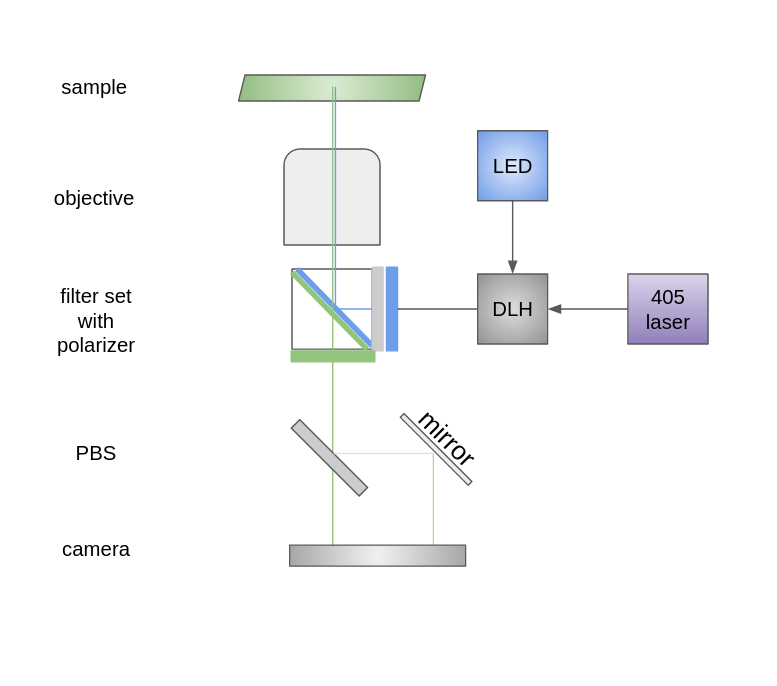
\includegraphics[trim=0 50 0 60,clip,width=0.8\linewidth]{figures/setup.png}\hspace*{\fill}}
    \caption{Fluorescence anisotropy imaging lightpath. A dual lamp housing (DLH) is used to introduce an LED light source for widefield excitation, and a 405nm laser for microirradiation, into the light path. Excitation light is polarized with a linear polarizer. Emission is collected and split with a polarizing beam splitter, which is then projected into the two halves of the camera.}
    {\label{fig:setup}}
\end{figure}

\paragraph*{} In such a setup, the effective field of view in the camera is reduced to halves, where the parallel and perpendicular component of the light is projected. To retrieve the components, I have written an image processing pipeline in python to automatically extract the parallel and perpendicular frames, and perform the anisotropy calculations on objects that might be detected in them. We use a frame reference, which is a bright field image, that highlights the edges of the aperture that separates the two components. We binarize the frame image, from which we segment out two intensity regions by overlaying it on top of our raw data. The segmented raw data is then registered with affine registration libraries, such that the pixels in both the channels correspond to each other in physical space.

\begin{figure}[!htp]
    {\hfill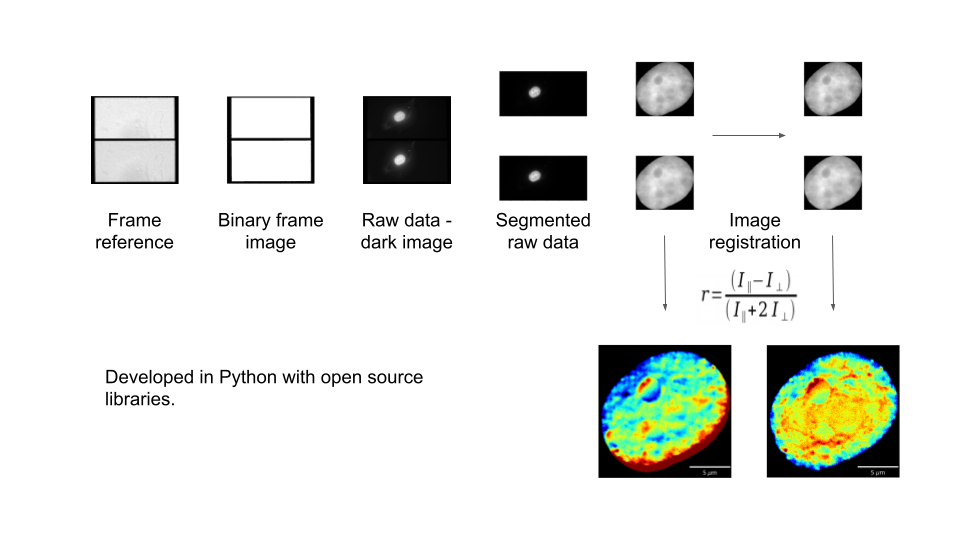
\includegraphics[clip,width=1\linewidth]{figures/pipeline.png}\hspace*{\fill}}
    \caption{Image analysis pipeline.}
    {\label{fig:pipeline}}
\end{figure}

\paragraph*{} To characterize the sensitivity of the system to changes in rotational correlation time, we varied the microviscosity of the dye fluorescein in water by increasing fraction of glycerol in the solution. This helped me in obtaining the Perrin's curve for the system, and helped determine the dynamic range of anisotropy values that the optical system is sensitive to. (Fig. \ref{fig:perrin})


\begin{figure}[!htp]
    {\hfill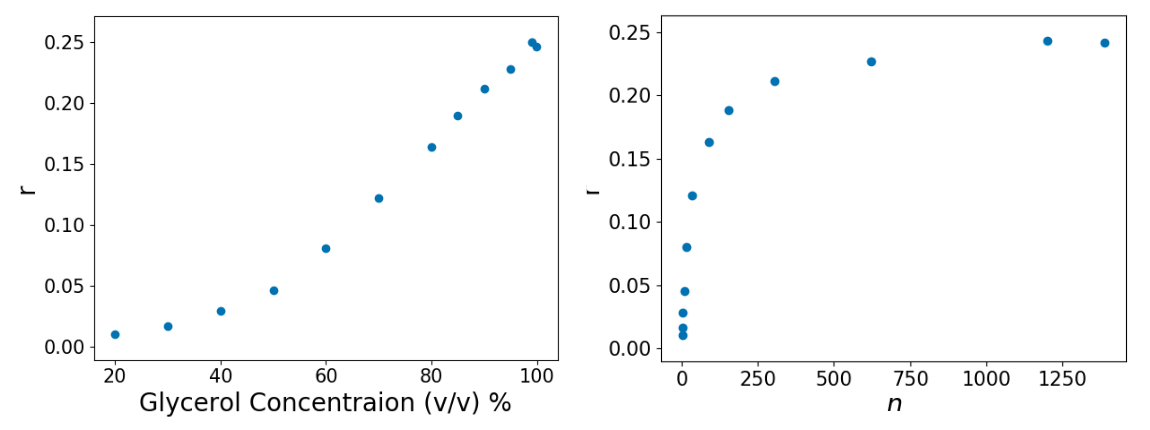
\includegraphics[clip,width=1\linewidth]{figures/perrin.png}\hspace*{\fill}}
    \caption{Perrin's curve for fluorescein in water with increasing glycerol concentration. A. Anisotropy is plotted against volume/volume fraction of Glycerol in water. B. The glycerol percentages are converted to calculated viscosity in centipoise.}
    {\label{fig:perrin}}
\end{figure}

\paragraph*{} The introduction of dual lamp housing (DLH) has the added advantage of introducing a laser in the light path of a widefield microscope, which can be used for the purpose of microirradiation, which has been used for inducing local damage on hoechst sensitized cells \cite{BURGESS20141703}. Using such a setup, we can study the physical effects on the chromatin structure with FAI, upon localized DNA damaged with microirradiation.

\section{Chromatin compaction maps}
\paragraph*{} In order to use this to map chromatin, core Histone, H2B, is tagged with EGFP and expressed in HeLa cells, which are then preferentially excited with polarized light, which maximally excites fluorophores whose excitation dipole are aligned to the polarization axis. The extent of depolarization of emission signal gives a measure of rotational diffusion of H2B-EGFP, which could be affected by its local environment. The higher the rotational diffusion, the greater is the extent of emission signal depolarizing. Anisotropy maps generated of H2B show that euchromatin like regions have greater rotational mobility than regions of heterochromatin, which is an evidence for differential packaging of chromatin compaction and can be used as a direct physical measure of chromatin packaging \cite{bhattacharya2009spatio}.

\begin{figure}[!hbtp]
    {\hfill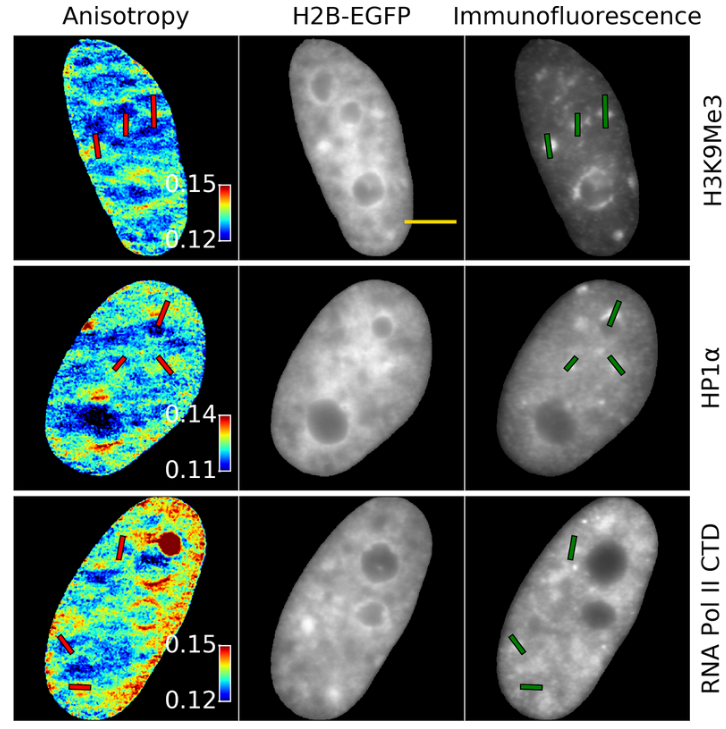
\includegraphics[trim=0 5 0 30, clip,width=0.8\linewidth]{figures/1.png}\hspace*{\fill}}
    \caption{H2B-EGFP anisotropy corresponds to known markers of heterochromatin and euchromatin. Immunofluorescence markers shown with anisotropy maps of fixed cells. HP1$\alpha$ and H3K9Me3 are known markers of heterochromatin, and phosphorylated RNA-Pol-II-CTD is a marker for active regions of transcription, where the chromatin is more open. Scale bar corresponds to 5$\mu$m.}
    {\label{fig:an_verify}}
\end{figure}

\begin{figure}[!hbtp]
    {\hfill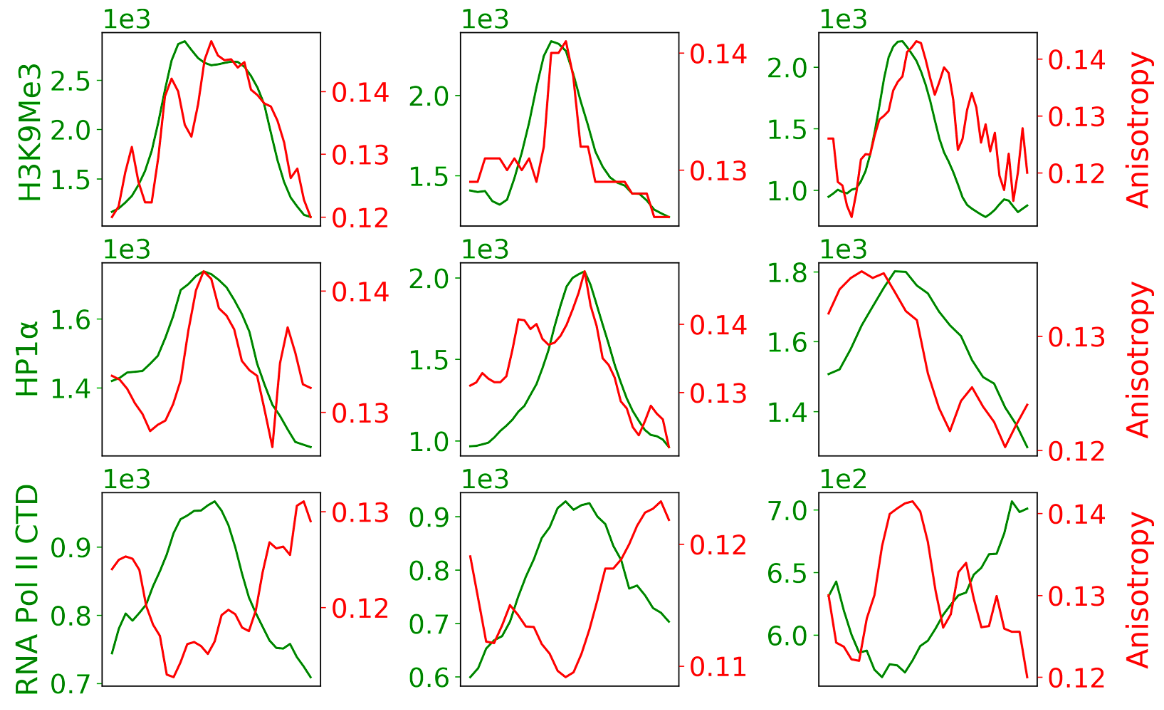
\includegraphics[clip,width=0.8\linewidth]{figures/2.png}\hspace*{\fill}}
    \caption{H2B-EGFP anisotropy corresponds to known markers of heterochromatin and euchromatin. Line profile of lines draw in the images in (Fig. \ref{fig:an_verify}) (green in immunofluorescence image, red in anisotropy map). Line profiles show that heterochromatin corresponds to regions of high anisotropy, while euchromatin corresponds to regions of low anisotropy. X-axis is distance along the line.}
    {\label{fig:an_verify_line}}
\end{figure}

\paragraph*{} In order to verify that the anisotropy values indeed correspond to biologically relevant structures of chromatin, we first demonstrated that anisotropy maps are preserved in fixation; we then imaged HeLa cells expressing H2B-EGFP for known markers of chromatin structures with immunofluorescence assay. We found that trimethylated lysine at ninth position in core Histone H3 (H3K9Me3), which is generally associated with densely packed heterochromatin regions correspond to high values of anisotropy (Fig. \ref{fig:an_verify}, \ref{fig:an_verify_line}). Similarly, we found that Heterochromatin Protein 1$\alpha$ (HP1$\alpha$), associated with heterochromatin domains, are also enriched in regions of high anisotropy. Conversely, we stained for decompacted chromatin using an antibody against the activated form of RNA polymerase, in which S5 is phosphorylated in C-terminal domain, and found that the anisotropy values are low in such regions. Together, these results suggested that regions of high and low anisotropy indeed correspond to biologically relevant structures of dense and loosely packed chromatin.  

\begin{figure}[H]
    {\hfill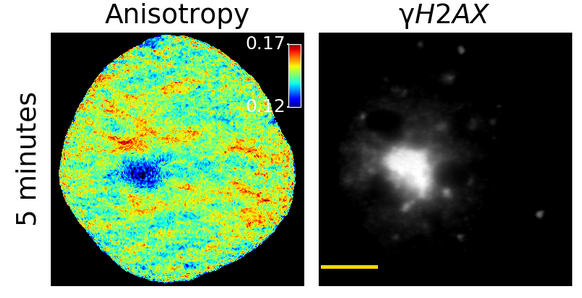
\includegraphics[clip,width=0.8\linewidth]{figures/micro_gh2ax.png}\hspace*{\fill}}
    \caption{Microirradiation activates DNA damage responses. $\gamma$H2AX, a known marker for damage response, is found at the site of microirradiation.}
    {\label{fig:micro_gh2ax}}
\end{figure}

\paragraph*{} To test that the 405nm laser that is introduced using the DLH is performing as intended, we focused the laser to a diffraction limited spot in the center of the image plane, and irradiated hoechst-sensitized cells. I observed that it causes damage by fixing the damaged cell within 5 minutes and staining the microirradiated cell for $\gamma$H2AX, which was observed at the site of damage (Fig. {\ref{fig:micro_gh2ax}}), indicating activated damage response.

\paragraph*{} In summary, we developed fluorescence anisotropy imaging to map regions of chromatin in live cells, verified its sensitivity and incorporated microirradiation to damage chromatin, and measure its dynamics post damage with live cell imaging. Following live cell imaging, we fixed the cells, and performed immunofluorescence assay against known markers of damage response to observe the state of those endogenous proteins.
